%manuals.tex
% user guides for software developed within VAMP (Vesicle Aspiration with MicroPipettes) project

\chapter{User Guides for Vesicle Aspiration with MicroPipettes (VAMP) project}\label{chap:userguide}

\section{LabVAMP - aspiration experiment automatization made with LabVIEW\copyright{}}\label{labvamp}

\subsection{What you can do with it}\label{labvamp-features}

With this software you can automate (to some extend) the experiments on aspirating the vesicles with micro-pipettes. In particular you can:
\begin{itemize}
	\item Control the position of 2 stages independently.
	\item Read outputs of two pressure sensors corresponding to these stages
	\item View real-time camera output and control it's zoom and pan.
	\item Save one image or a series of images (with no definable frame rate, just as fast as possible) to the directory of your choice.
	\item Perform scanning through user defined pressure sets (independent for 2 stages), with definable timeout after reaching desired stage positions (to let the pressure reach the pipette and equilibrate) together with number of images to make for each pressure and time gap between these images (for later averaging purposes).
\end{itemize}

\subsection{User Interface}\label{labvamp-ui}

\begin{figure}[htbp]
	\centering
		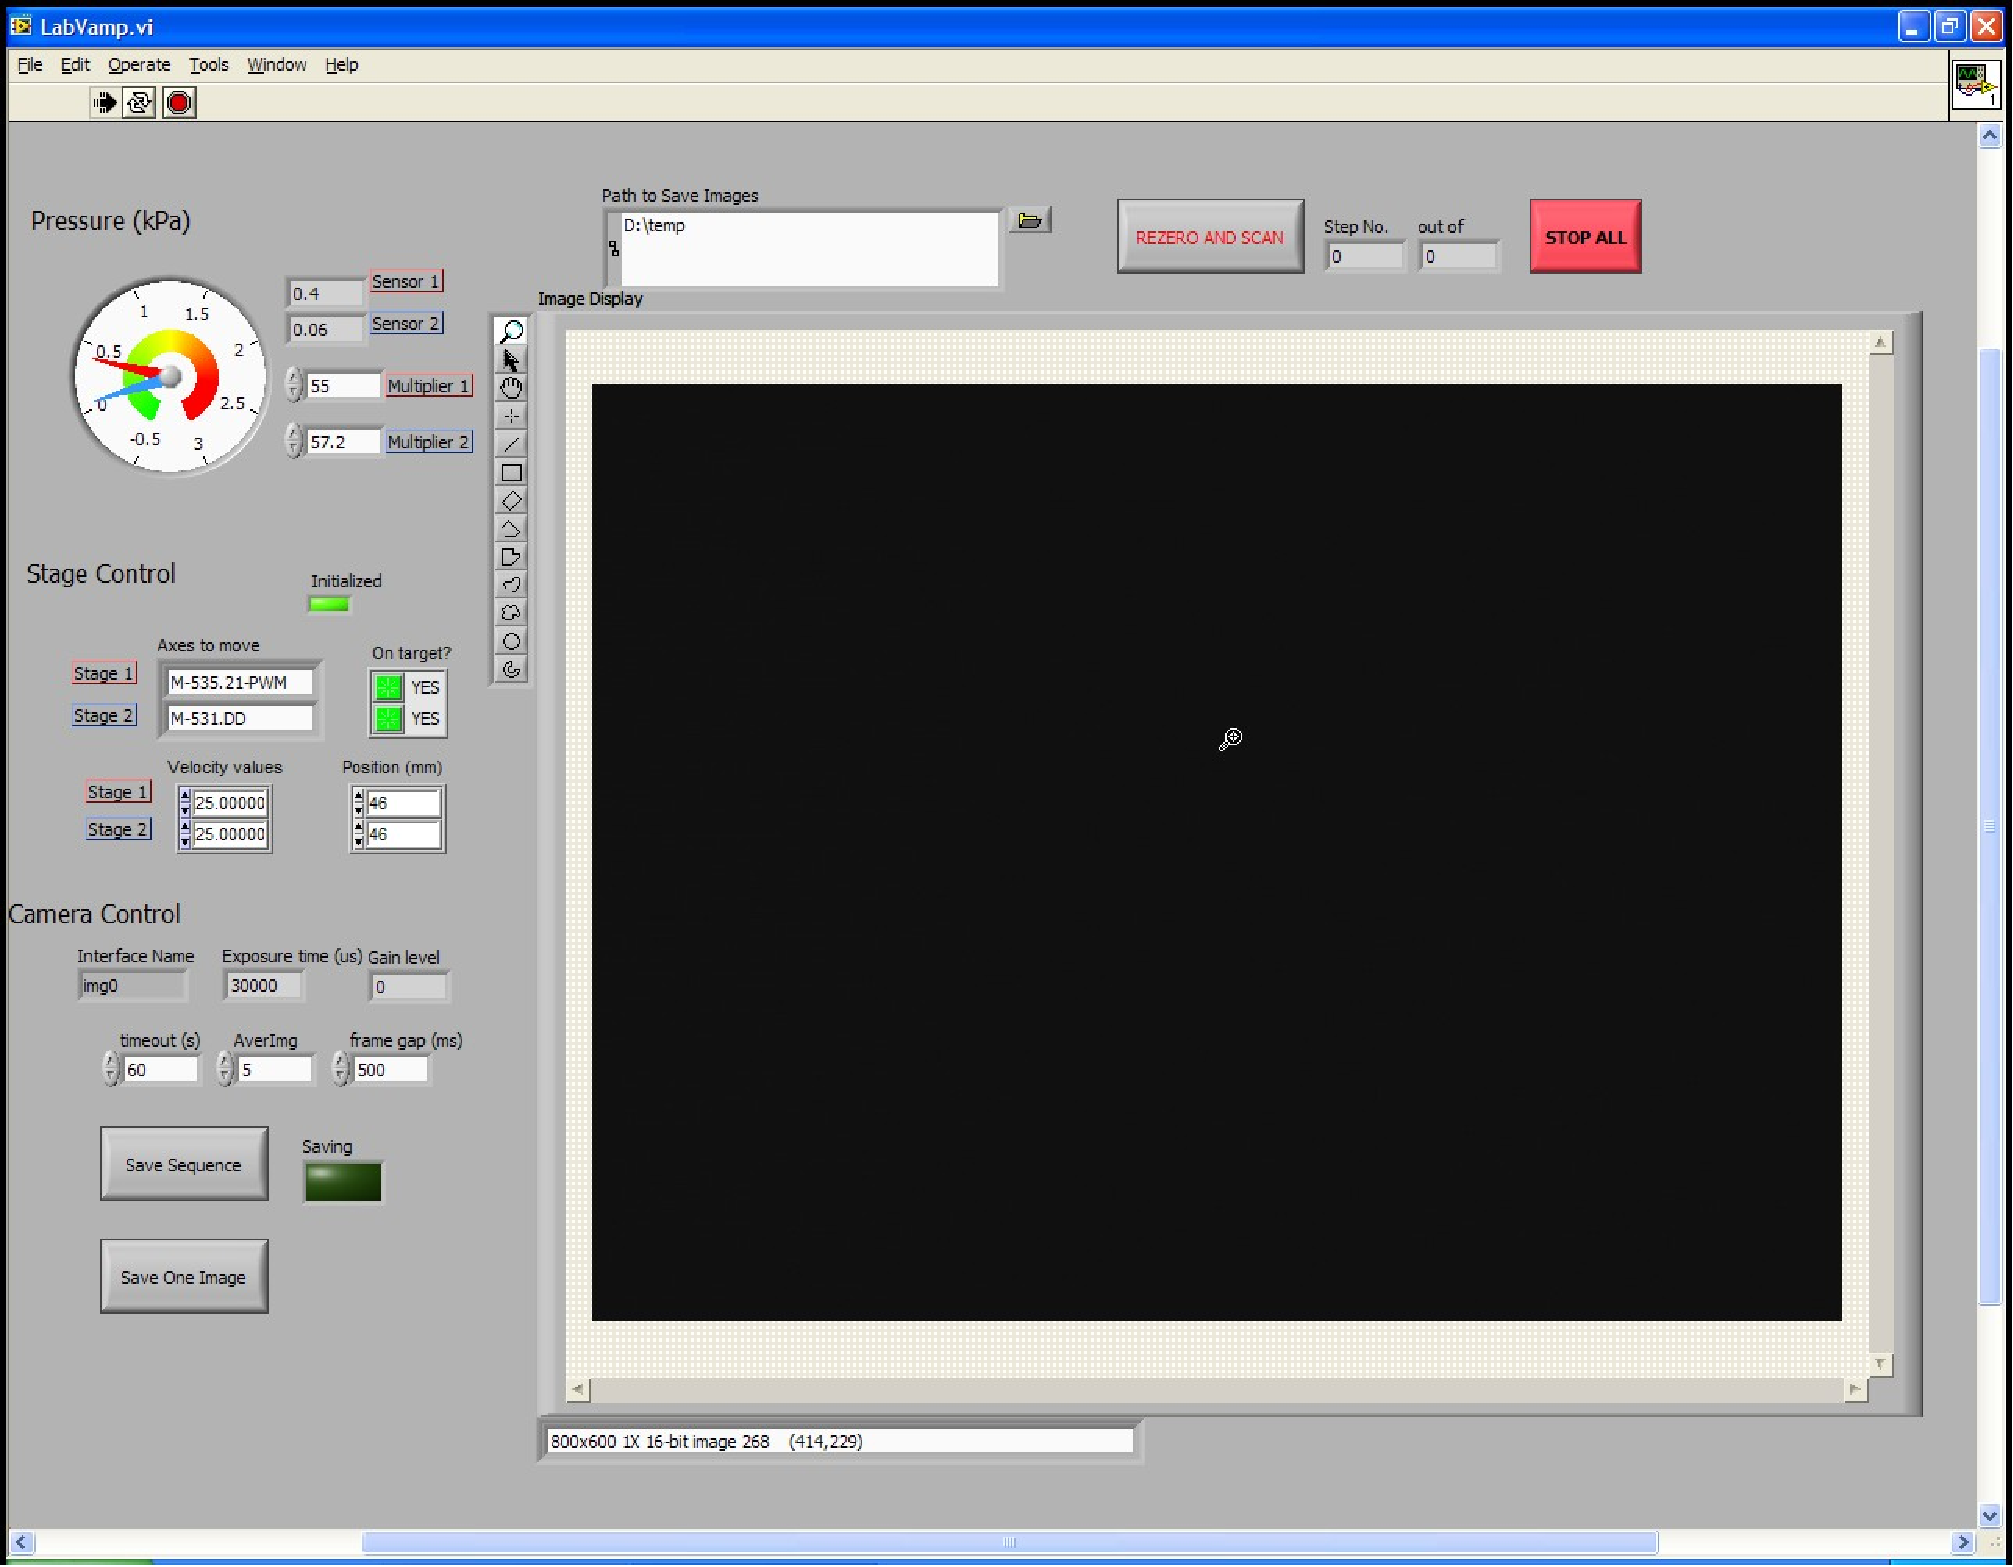
\includegraphics[width=1.00\textwidth]{figs/labvamp_ui.pdf}
	\caption{LabVAMP User Interface}
	\label{fig:labvampui}
\end{figure}

\begin{enumerate}
	
	\item Image display unit:
	
	\begin{figure}[htbp]
		\centering
			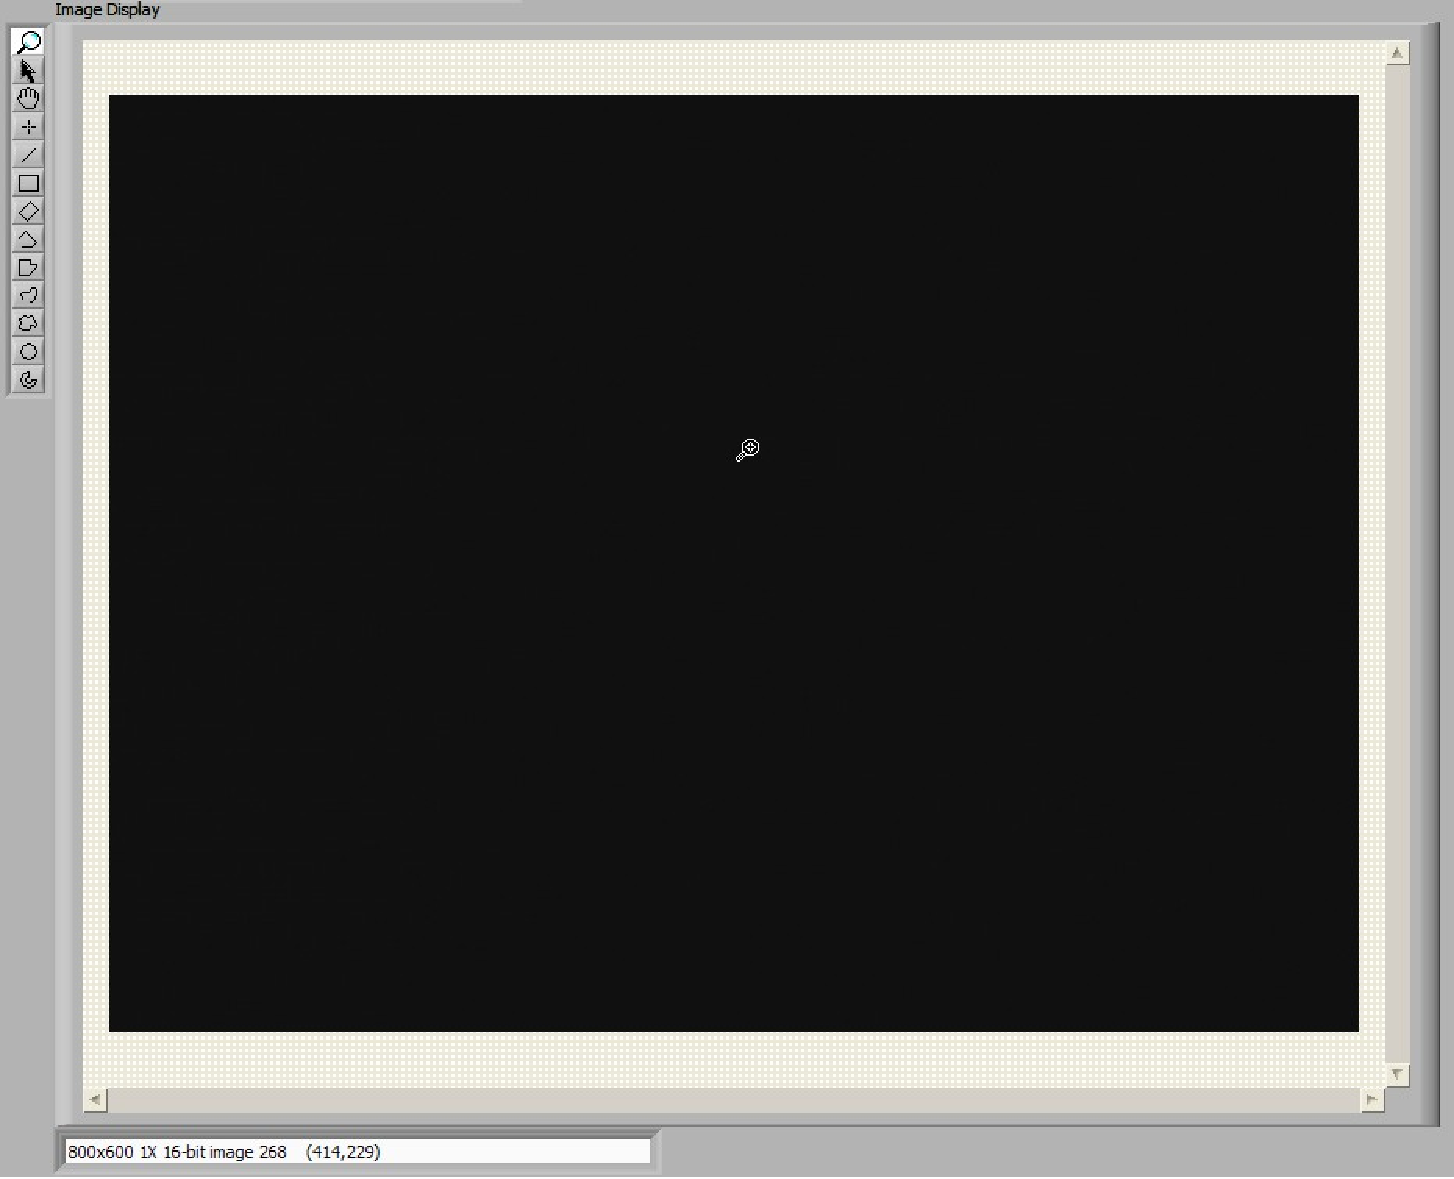
\includegraphics[width=1.00\textwidth]{figs/labvamp_imgdisplay.pdf}
		\caption{Image Display Unit}
		\label{fig:LabVAMP_imgdisplay}
	\end{figure}
	
	\begin{enumerate}
		\item Image window, showing the live image from the camera
		\item Image tools palette. You are interested in first and third tools - zoom tool and pan tool (other features are not implemented). Zoom tool allows you to zoom in and out of the image by clicking and SHIFT-clicking respectively (the cursor will change accordingly). Pan tool allows you to drag the zoomed image without use of scrollbars.
		\item Image status bar, displays resolution of the image, current level of zoom and current pixel brightness value under the cursor.
	\end{enumerate}
	
	\item Pressures display unit:
	
\begin{figure}[htbp]
	\centering
		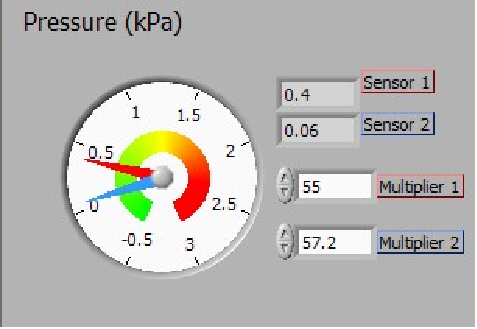
\includegraphics{figs/labvamp_press.pdf}
	\caption{Pressures Display Unit}
	\label{fig:LabVAMP_press}
\end{figure}
	
	\begin{enumerate}
		\item Pressure readings, in kPa. Items are color-coded together with stage numbers.
		\item Pressure sensors multipliers. These are values for converting from readings of pressure transducers (in V) to pressures (in kPa), defined while calibrating the sensors. Zero shift is not accounted for since only change in pressure has a meaning in this experiment.
	\end{enumerate}
	
	\item Stages control unit:
	
	\begin{figure}[htbp]
		\centering
			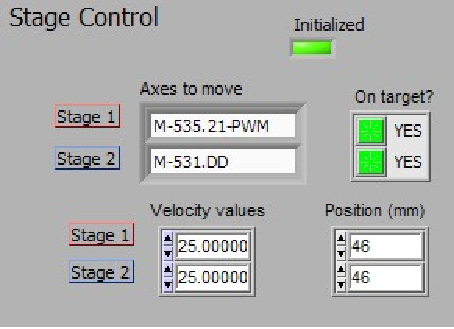
\includegraphics{figs/labvamp_stages.pdf}
		\caption{Stages Control Unit}
		\label{fig:LabVAMP_stages}
	\end{figure}
	
	\begin{enumerate}
		\item Stage names as defined by C-843 controller card configuration file.
		\item ``Init'' LED - is lit when both stages have been initialized and are ready to accept commands.
		\item Velocity control - controls how fast stages are moving (in $mm/sec$).
		\item Position control - controls position of stages (in mm). Note that $1~mm$ of water equals to $9.81~Pa \approx 0.01~kPa$
		\item ``On Target'' LEDs - indicate that respective stage has arrived at the position defined by position control.
	\end{enumerate}
	
	\item Camera control unit:
	
	\begin{figure}
		\centering
			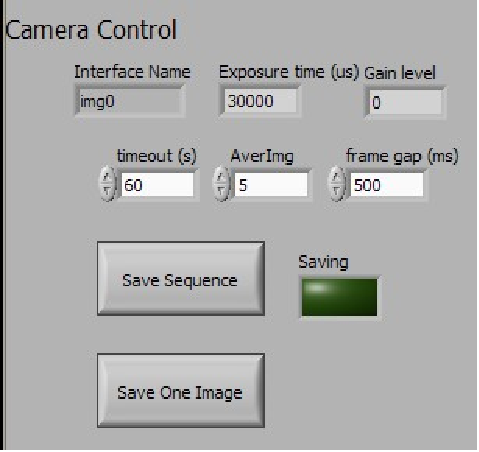
\includegraphics{figs/labvamp_cam.pdf}
		\caption{Camera Control Unit}
		\label{fig:labvamp_cam}
	\end{figure}

	\begin{enumerate}
		\item Camera information - current camera interface name (as defined by LabVIEW), exposure time and gain value.
		\item Scan settings:
		\begin{enumerate}
			\item ``Timeout'' - time to wait after arriving at target position before making snapshots
			\item ``AverImg'' - how many images to make for each pressure protocol item
			\item ``Frame Gap'' - time between making snapshots for one pressure protocol item.
		\end{enumerate}
		\item Manual image saving:
		\begin{enumerate}
			\item ``Save one'' button - saves one image in the defined folder, with predefined file naming scheme (see \ref{labvamp-work}).
			\item ``Save Seq'' button - saves a sequence of images in the defined folder with predefined file naming scheme (see \ref{labvamp-work}).
			\item ``Saving..'' LED - indicates that the sequence of images is being saved.
		\end{enumerate} 
	\end{enumerate}
	
	\item Scan Control Unit:
	
	\begin{figure}[htbp]
		\centering
			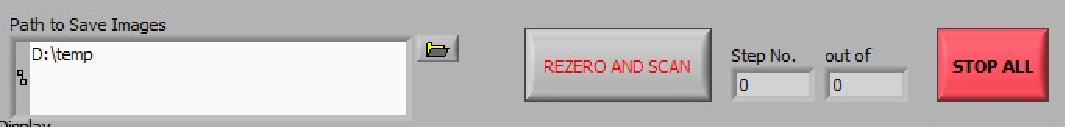
\includegraphics[width=1.00\textwidth]{figs/labvamp_scan.pdf}
		\caption{Scan Control Unit}
		\label{fig:LabVAMP_scan}
	\end{figure}

	\begin{itemize}
		\item Image folder - allows you to choose where to save images.
		\item ``Rezero/Scan'' button - remembers the current position(pressure) as a zero and starts scanning of the pressure range (see \ref{labvamp-work}).
		\item ``Step.. from...'' - indicates the position in pressure protocol being processed.
		\item ``STOP ALL'' button - cancels current operations and exits the program. Mind the limitations \ref{labvamp-limits}!
	\end{itemize}
\end{enumerate}

\subsection{Work flow}\label{labvamp-work}
\begin{enumerate}
	\item Launch camera dedicated driver to tune all the parameters needed (image size, exposure, gain). Close the driver software.
	\item Launch LabVAMP. The picture from the camera will appear. The stages will begin to move while initializing. Meanwhile you can enter the rough estimate for initial position in the position fields - stages will move to this position when having initialized. The LEDs ``Initialized'' and ``On Target'' indicate, correspondingly, the state of the stages and whether the stage is in position set by ``Positions'' control.
	\item When the ``Initialized'' and ``On Target'' LEDs are lit, you can start the experiment.
	\item To save a single image, choose a directory where to save them, and press ``Save One'' button. The image will be saved in the chosen directory as PNG file with filename denoting the time the image was saved with microseconds precission (HH-MM-SS.XXX.png).
	\item To save the sequence of images choose the directory where to save them and press ``Save Seq'' button. The button remains pressed, and the ``Saving'' LED is on. To stop saving sequence press ``Save Seq'' button again so it looks depressed. Mind the limitations noted in \ref{labvamp-limits}. Images are saved with the same file name scheme as with single snapshots.
	\item To move stages adjust the position and velocity inputs and observe changes on pressure readings. Pressure values (numbers and arrows) are color-coded with corresponding stages. The output is in kPa with 2 decimal digits since it is roughly the accuracy of the pressure sensor itself (approx 8 Pa).
	\item Please note, that pressure sensor \emph{does not} show the pressure applied to the pipette. It shows the pressure arising from different hight of movable and unmovable reference water vessels. Hence, with pressure sensor you should observe the \emph{difference} in pressures.
	\item To perform automatic scanning of a pressure range:
	\begin{enumerate}
		\item Prepare the pressure protocol file. This must be a simple ASCII text file with 2 columns (TAB separated) of pressure values \emph{in Pa}. Each column corresponds to one stage, and so each row corresponds to one particular position of stages, and hence pressures applied to both pipettes and recorded with camera afterwards. Please note that these pressures will be applied \emph{relative} to some ``zero''-value you will choose in the course of the experiment. If you will use only one stage, fill values for another one with zeroes.
		\item Adjust the pressure in the pipette(s) so that the vesicle(s) is merely hold. This will be you zero-pressure when supposedly the tension is as close to the unperturbed state as possible.
		\item Adjust the ``timeout'' value, which is how long the program will wait after the stages arrived at desired position during scan before making any snapshots. This is to ensure that pressure has indeed reached the pipette mouth and equilibrated - in some situations (like very thin pipette) this can take quite long, so you better first play with the stages to make some estimation of this parameter.
		\item ``AverImg'' and ``Frame gap'' are used to make several snapshots for each position in pressure protocol to get semi-subpixel resolution afterwards by averaging between the images. AverImg is thus the number of images to take for every protocol position and ``frame gap'' is time between these snapshots.
		\item If you haven't done it so far (or if you want to change it) choose the directory where the images will be saved.
		\item Press ``Rezero/Scan'' button. You will be asked for the location of pressure protocol file you created earlier. After you choose the file, the scan will commence, with number of current row processed being indicated as ``Step''.
		\item Images are saved in the directory chosen as PNG images (for the TELI DCL3690 TIF-format was ruled out since most software apparently can not adequately cope with 12-bit TIF generated by LabVIEW), with the following naming scheme:\\ \emph{[number of step]-[pressure on stage 1]-[pressure on stage 2]\_[index of AverImg].png}.
		\item Mind the limitations of the program! \ref{labvamp-limits}
	\end{enumerate}
\end{enumerate}

\subsection{Limitations}\label{labvamp-limits}
Currently LabVAMP has the following limitations:
\begin{itemize}
	\item The actual camera setup must be made \emph{before} LabVAMP is launched, with camera original drivers. LabVAMP merely shows some current relevant camera settings, like shutter speed, gain level and image resolution. The LabVAMP \emph{and} camera drivers \emph{can not be run simultaneously}.
	\item the actual frame rate you get when saving sequence of images does heavily depend on the image parameters. If it is the full scale image (1280x1040 for TELI CS-3960DCL) then the frame rate is of the order of 7 fps, but for VGA images (640x480) (and probably for SVGA also) it is already close to technical limits of the camera, i.e. 30 fps.
	\item The pressure readings are currently absolute (not re-zeroed) and are more of cosmetic type - they are not used in actual calculation of stage positions.
	\item When the software is launched the stages will move, probably by the whole range (depending on the stage), as a part of initialization, thus applying pressures to pipettes, so operate the pipettes after the LabVAMP is launched (or close the pipette valve before launching and choose wisely the initial stage positions).
	\item After the scan is started, the process can not be interfered - pressing STOP ALL button will  stop the outputs of camera and pressure sensor at once (and thus the saving of images), and the stage will continue scanning/waiting until the current step in pressure protocol complete. Also the scan control values (timeout etc) and stage settings (like speed) are frozen at the beginning of the scan, so they can not be changed afterwards. You can of course close the whole program by hand, but then you will leave the hardware in unknown state and very likely will need to access the hardware (pressure sensor, camera and stages) first by their native drivers before launching LabVAMP again, otherwise you might get an error and/or crush the program.
	\item After the scan is complete, the final dialog asks about quitting the program. If you answer NO, LabVAMP will only continue showing you the output of the camera, but you will not be able neither to move stages, nor save images, let alone start a new scan. To repeat the process the program should be shut down (by pressing STOP ALL) and restarted.
\end{itemize}

\section{VAMPy - aspiration image analysis made with Python}\label{vampy}
\emph{Being in active development, the state of the program might be quite different from what is written here!}

As it is now (not packaged in self-contained executable) you need the following software to be installed on your computer to run VAMPy:
\begin{itemize}
	\item Python 2.6.6 (\url{http://www.python.org}
	\item NumPy 1.5 (\url{http://www.scipy.org}
	\item SciPy 0.8 (\url{http://www.scipy.org}
	\item matplotlib 1.00 (\url{http://matplotlib.sourceforge.net/})
	\item wxPython 2.9.11 (\url{http://www.wxpython.org}
	\item Python Image Library 1.1.7 (\url{www.pythonware.com/products/pil/}) 
\end{itemize}
All of the above is Open Source and freely available from respective websites. Version numbers are the ones with which the software was developed and tested, but it might also work with older versions and hopefully will work with future versions of Python language and packages. The program is cross-platform, it runs on Windows (tested), Linux/Unix (tested) and Mac (not tested) as long as all dependencies are met.

\subsection{What you can do with it}\label{vampy-features}
\emph{Warning: list of features is actively changed!}

Currently you can:
\begin{itemize}
	\item Open images of aspirated pipette and view them as stack of images.
	\item Crop the unnecessary parts of the image, rotate it as needed and save this settings for future reuse.
	\item Load corresponding pressure file or read pressures from image filenames.
	\item Analyze the geometry of the image and obtain plots for total area of the vesicle, its volume etc.
	\item Check suspicious points by analyzing single images to see whether the image analysis succeeded.
	\item Obtain the plot of tension vs dilation and corresponding value for the bending rigidity or stretching elasticity from fitting of data.
	\item Export results of geometry analysis and tensions calculations to ASCII file.
	\item Load manually measured geometry data and applied pressure from text files, calculate corresponding dilations and tensions and fit them for getting bending rigidity and stretching elasticity.
	\item As the above but load already manually calculated tensions and dilations from text file.
\end{itemize}

\subsection{User Interface}\label{vampy-ui}
\begin{itemize}
	\item Main window (figure \ref{fig:vampymain})
		\begin{figure}[htbp]
			\centering
			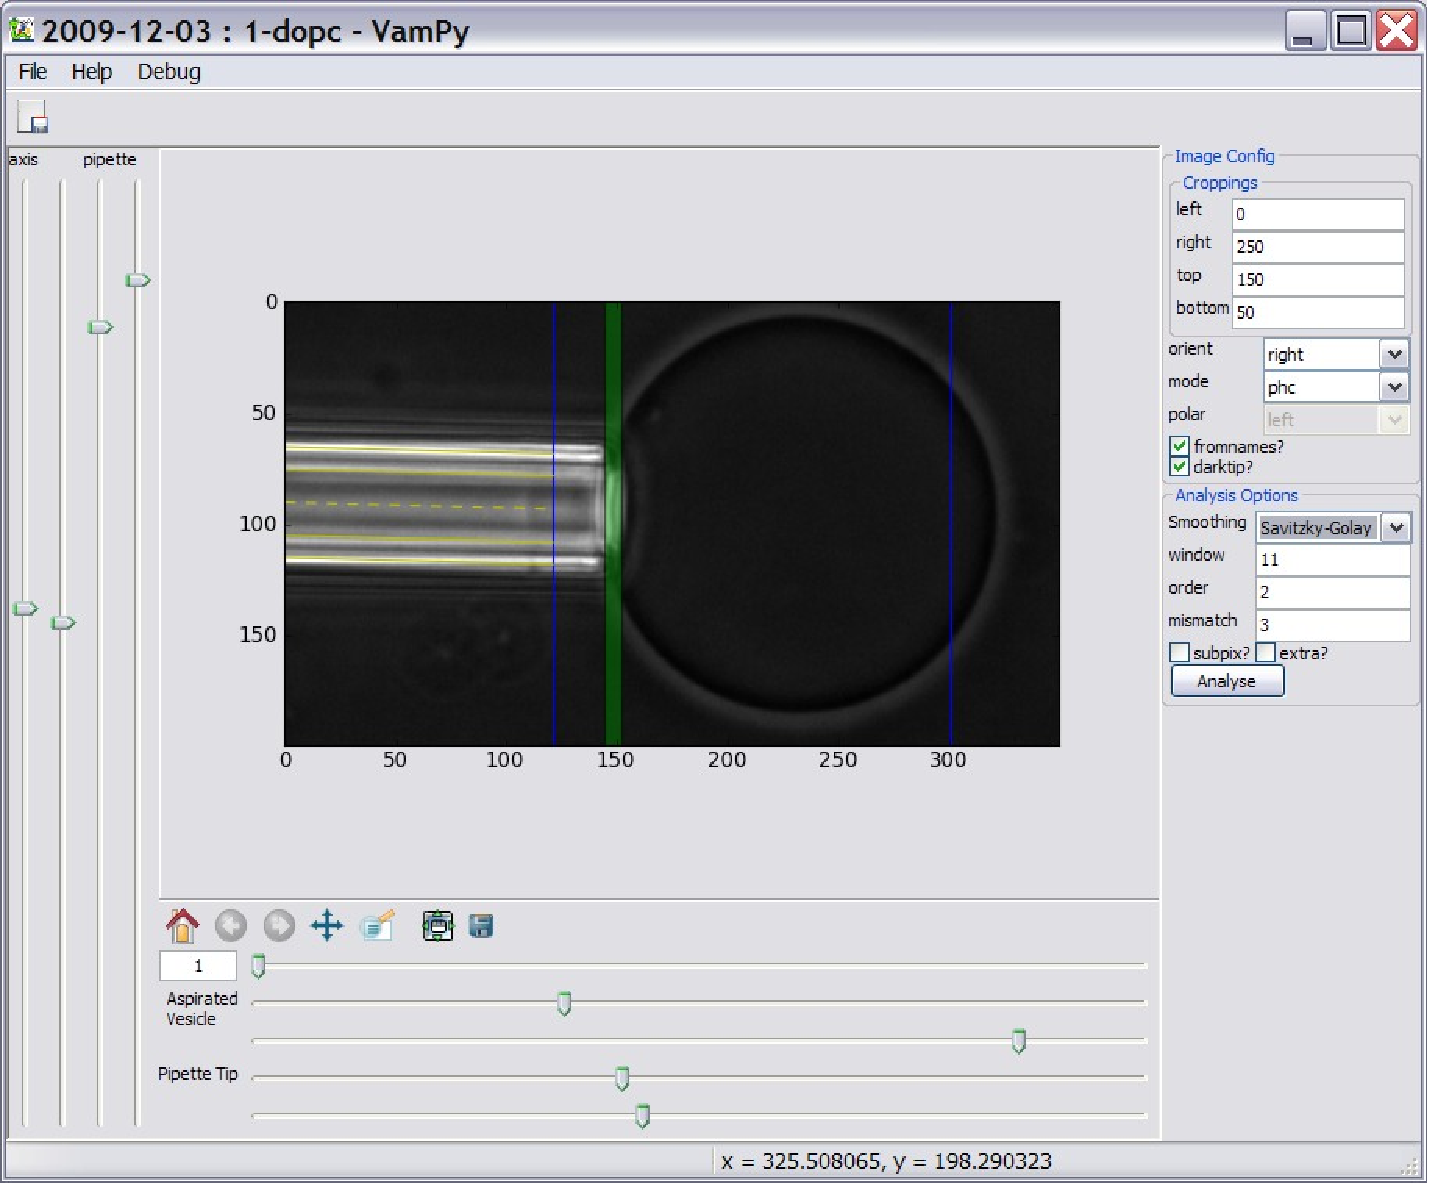
\includegraphics[width=1.00\textwidth]{figs/vampymain.pdf}
			\caption{VAMPy main window}
			\label{fig:vampymain}
		\end{figure}
		\begin{enumerate}
				\item Menu Bar - quite self-explanatory
					\begin{itemize}
						\item File - open directory, exit application
						\item Help - About info, Help (not implemened yet, shows the same info as ``About''
						\item Debug - Debug single image (for analysing image recognition performance), reload (for developers - reloads math modules without restarting GUI)
					\end{itemize}
				\item Tool Bar - contains buttons for some actions (``Open images folder'' and ``Save image config'')
				\item Image panel:
					\begin{enumerate}
						\item Image with region lines and pipette lines
						\item Image toolbar (zoom, pan, adjust subplots, go back and forward between views, save plot as image - does not affect analysis, only representation)
						\item Image slider - scrolls through the images
						\item Region sliders - control region lines for aspirated tip, outer vesicle and pipete mouth
						\item Axis sliders - control the estimation of the pipette axis position
						\item Pipette sliders - control the estimation (radius and walls thickness) of pipette position
					\end{enumerate}
				\item Image Config panel
					\begin{enumerate}
						\item Croppings - used to crop the image
						\item Orientation - for rotation the image
						\item Mode - type of the image (phase contrast or dic)
						\item Polar - type of the dic image
						\item fromnames - how to load pressures, from images filenames (checked) or from pressure file (unchecked)
						\item darktip - what to count for pipette mouth, brightest(unchecked) or the darkest (checked) pixels
					\end{enumerate}
				\item Analsis Options panel
					\begin{enumerate}
						\item Smoothing -- type of applied smoothing (Savitzky-Golay or Gauss readily available)
						\item window - full window size for the smoothing filter (odd integer since point plus same number of points to the left and to the right)
						\item order - used for smoothing the image while processing (polinomial order for Savitzky-Golay, blurring strength for Gauss)
						\item mismatch - the maximal difference between pixel and subpixel resolution to tolerate subpixel routine as successful \emph{(not implemented yet, ignored)}
						\item extra - output extra information as NumPy saved arrays (NPZ) and python pickles \emph{(not implemented yet, ignored)}
						\item subpixel - use subpixel resolution \emph{(not implemented yet, ignored)}
						\item Analyse - start processing 
					\end{enumerate}
				\item Status Bar - when the cursor is in the image/plot shows current coordinates 
		\end{enumerate}
	\item Geometry window (figure \ref{fig:vampygeom})
		\begin{figure}[htbp]
			\centering
			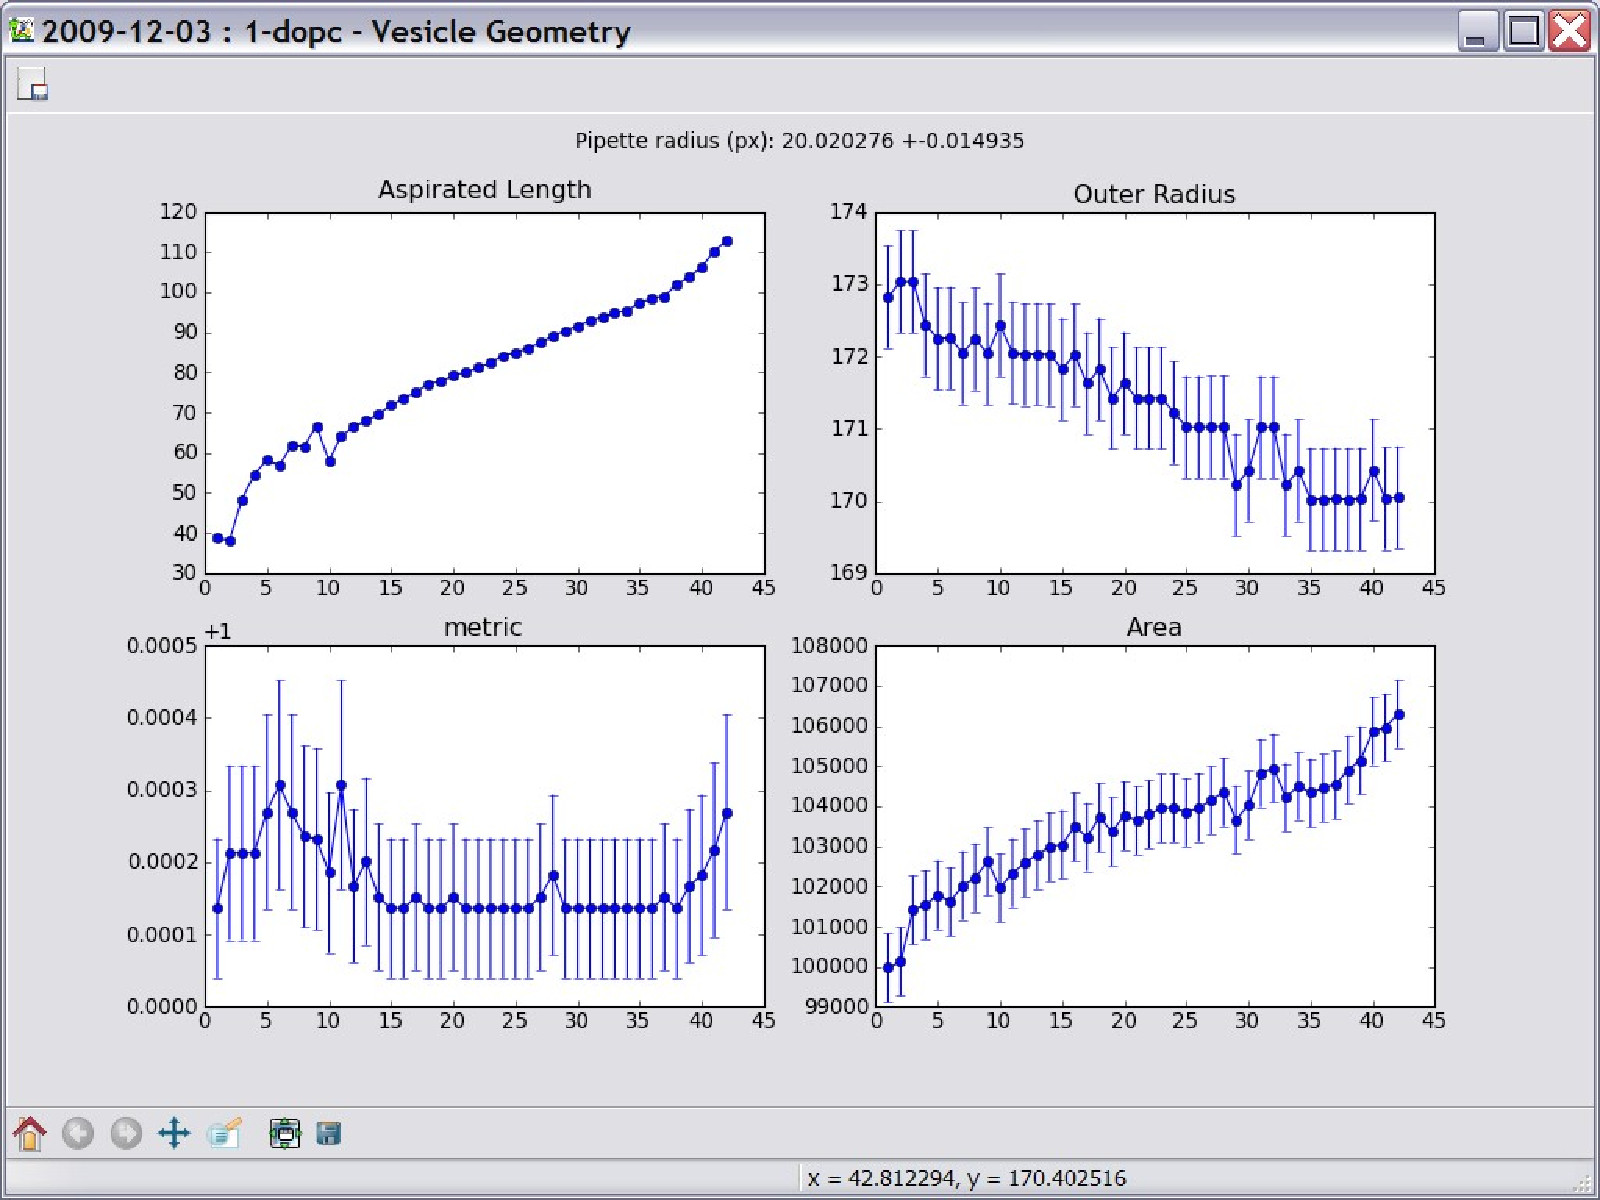
\includegraphics[width=1.00\textwidth]{figs/vampygeom.pdf}
			\caption{VAMPy vesicle geometry window}
			\label{fig:vampygeom}
		\end{figure}
		\begin{enumerate}
			\item Toolbar - buttons to open external geometry file and to save all the calculated data to the ASCII file
			\item Plots - plots of various calculated parameters - currently aspirated length, outer vesicle radius, vesicle total volume and metric (related to the tilt of the axis with 1 being perfectly horizontal). Calculated pipette inner radius is also displayed.
			\item image toolbar - the same as on main window
			\item status bar - the same as on main window
		\end{enumerate}
	\item Fitting window (figure \ref{fig:vampyfit})
		\begin{figure}[htbp]
			\centering
			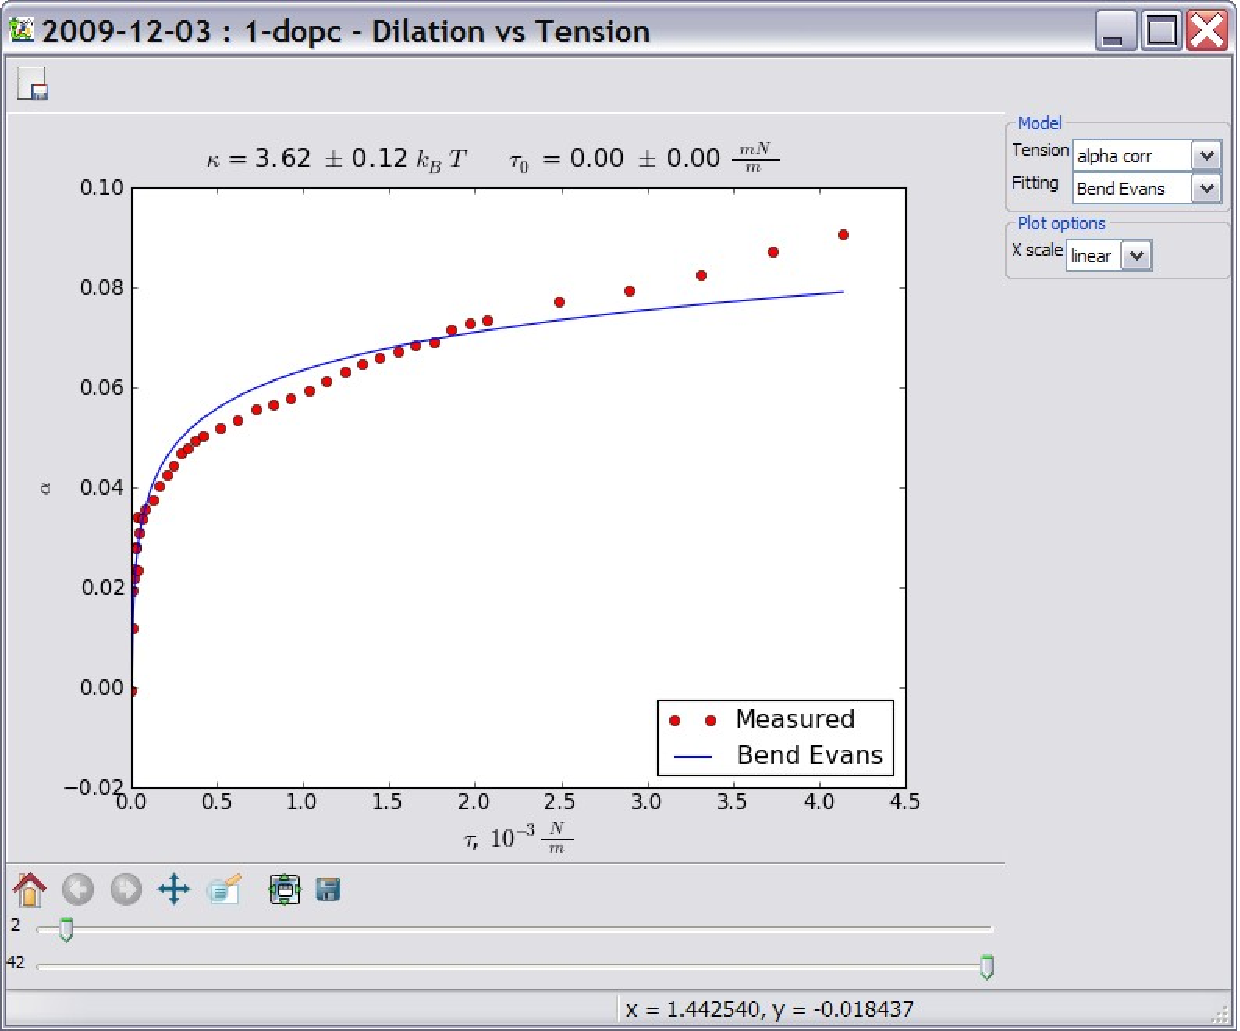
\includegraphics[width=1.00\textwidth]{figs/vampyfit.pdf}
			\caption{VAMPy fitting window}
			\label{fig:vampyfit}
		\end{figure}
		\begin{enumerate}
			\item toolbar - buttons to open external file with tensions/dilations and to save calculated tensions and dilations to ASCII file (for example to analyse/fit it with other tools)
			\item plot of the dilation vs tension - both experimental points and fitted line are shown, with fitted values printed on top
			\item range slider - choose what range of values to fit
			\item Model parameters
				\begin{enumerate}
					\item Tension model used for calculation of tensions/dilations
					\item Model to fit data with
				\end{enumerate}
			\item plot options - currently only choice for x coordinate as linear or log10
			\item image toolbar - the same as on main window
			\item status bar - the same as on main window
		\end{enumerate}
	\item Debug window (figure \ref{fig:vampydebug})
		\begin{figure}[htbp]
			\centering
			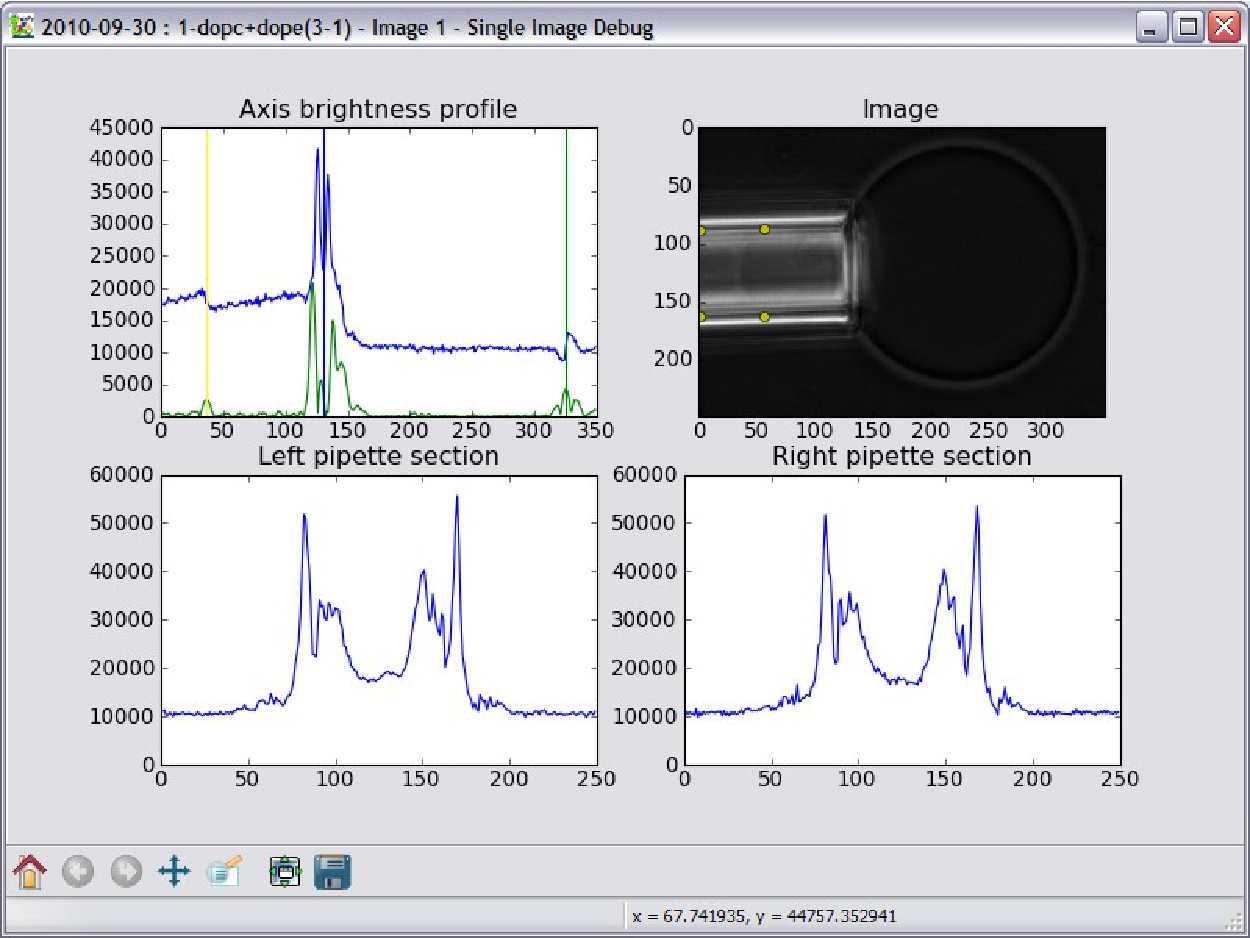
\includegraphics[width=1.00\textwidth]{figs/vampydebug.pdf}
			\caption{VAMPy single image debug window}
			\label{fig:vampydebug}
		\end{figure}
		\begin{enumerate}
			\item plot of various values for the single chose image - currently axis brightness profile and absolute value of its smoothed derivative with found features positions, found positions of pipette walls, brightness profile across pipette used to find pipette walls
			\item image toolbar - the same as on main window
			\item status bar - the same as on main window
		\end{enumerate}
\end{itemize}

\subsection{Work flow}\label{vampy-work}
\begin{enumerate}
	\item If it is the first time you run the software on this particular computer, make sure that all dependencies are installed (see \ref{vampy}).
	\item Run the program by launching file ``VamPy.pyw'' (on Windows) or from command line 'python VamPy.pyw' (Linux/Unix)
	\item Open desired folder with images to analyze (Menu$\rightarrow$File$\rightarrow$Open... or Ctrl+O or Toolbar button). You will also be prompted for file type to load (currently only PNG or TIF images are supported).
	\item If the folder contained a file ``vampy.cfg'', the program will try to load image settings (cropping, rotation) and sliders positions from it.
	\item Crop the image as desired - the smaller the image, the faster program works and less noise/artifacts it might encounter while analyzing images. You can use image slider to scroll through images and make sure that you do not crop out any significant parts. Sides of cropping are relative to original image
	\item Rotate image so that \emph{pipette sticks from the left side}. This is very important!
	\item Choose the type of image you are analyzing - phase contrast or differential contrast. For latter, choose also ``polar'' parameter, which is the side from where a ``virtual light'' is shining in your picture - if the left part is bright and the right has ``shadows'', choose ``left'' and vice versa.
	\item Check the option 'fromnames' if the pressures must be read from image filenames (as created with LabVAMP program). If not, the pressure file used for the experiment will be asked for
	\item decide for what will be counted as pipette mouth - it can be either a most bright part in the region of the pipette mouth or the most dark one ('darktip' unchecked or checked respectively) - ideally pipette tip produces a dark line, but with small pipette/bright illumination it might be blurred already beyond recognition, so you will have to define the pipette tip from the brightest pixels
	\item Adjust region, axis and pipette sliders so that on every image in the stack:
	\begin{itemize}
		\item Dashed line goes approximately along the pipette axis
		\item The darkest part of the pipette walls is always inside the estimation for pipette walls (yellow lines)
		\item The tip of the aspirated part is always to the left of the left vertical blue line
		\item The outer vesicle part crossing the pipette axis is always to the right of the right blue line
		\item The green region is as narrow as possible but always covering the pipette mouth
	\end{itemize} 
	\item You can save image settings - crop, rotation, position of sliders etc to use them next time you open these images, just press ``Save image info'' button in the toolbar. Settings will be saved as a simple tab separated ASCII-file ``vampy.cfg'' in the folder from where current images were loaded.
	\item Other parameters that affect the analysis:
	\begin{itemize}
		\item ``smoothing'' - what algorithm to use for smoothing and derivating the brightness profile
		\item ``window''- full width of the window in the smoothong filters that need it, otherwise ignored
		\item ``order''- smoothing strength, has different meaning in different filters (for example polinomial order in Savitzky-Golay, strength of blur in Gaussian)
		\item ``Extra'' - return a lot of additional info from image analysis and save them to external files (not fully implemented yet)
		\item ``Subpix'' - check to have a fitting routines for subpixel resolution (not fully implemented yet).
		\item ``Mismatch'' - determines when to discard the subpixel value for pixel value (as with subpixel resolution itself, not fully implemented yet).
	\end{itemize}
	\item Press the ``Analyse'' button. If you haven't checked ``fromnames'' check box, you will be prompted for the location of the pressure protocol file.
	\item The program automatically determines the situation when there are more than one image for each pressure and handles it correctly if all images are present, otherwise it produces an error message.
	\item In any case in the next dialog you will also be prompted for the next parameters:
	\begin{itemize}
		\item Stage number - which column in the pressure protocol file (part of the name of the image file) to use as a pressures for these images.
		\item Scale factor - conversion from pixels to micrometers, can be measured with the microscope ruler. Default value is for TELI CS-3960DCL camera and overall magnification of 20X.
		\item Pressure accuracy - needed for the calculation of tension accuracy (and thus accuracy of output parameters of fitting), determined by the accuracy of the stages moving the water vessels. Default is for PI M-535.21 linear stage.
	\end{itemize}
	\item After some processing time two windows will pop out - ``Vesicle Geometry'' and ``Dilation vs Tension''
	\item ``Vesicle Geometry'' shows you values and plots of various extracted/calculated parameters already averaged between images corresponding to the same pressure, such as measured pipette diameter, total vesicle volume, area, outer vesicle radius etc  .
	\item ``Dilation vs Tension'' window presents the corresponding plot together with its fit with one of the chosen models/algorithms, with fitted value printed on top of the plot.
	\item By using sliders you can control the region which is fitted.
	\item You can also inspect how well the image recognition worked on any particular image by choosing ``Debug$\rightarrow$Debug image'' from the menu of the main window. The Debug window will open, allowing you to check the algorithm performance.
\end{enumerate}

\subsection{Limitations}\label{vampy-limits}
Current problems/limitations/target for improvements:
\begin{itemize}
	\item Not thoroughly tested for dic-images
	\item No subpixel resolution for single images
	\item No extra data available to user
\end{itemize}